\begin{pastexam}[label={px:ncku-113-prog-06}]{成大資訊聯招 113 學年度 第 6 題}
（單選）

\textbf{[5\%]} Given the following height-based leftist tree.
\begin{center}
\begin{tikzpicture}[x=0.0145cm,y=-0.0145cm,wn/.style={ellipse,draw,fill=white,inner sep=0pt,minimum width=0.8cm,minimum height=0.52cm,font=\sffamily\bfseries\small},bn/.style={wn,fill=black,text=white}]
\node[wn] (n4) at (718,869) {4};
\node[wn] (n9) at (600,937) {9};
\node[wn] (n7) at (822,937) {7};
\node[wn] (n16) at (535,998) {16};
\node[wn] (n14) at (665,997) {14};
\node[wn] (n10) at (766,998) {10};
\node[wn] (n16b) at (882,996) {16};
\node[wn] (n18) at (488,1062) {18};
\node[wn] (n21) at (569,1062) {21};
\node[wn] (n17) at (630,1062) {17};
\node[wn] (n15) at (727,1062) {15};
\node[wn] (n12) at (802,1062) {12};
\node[wn] (n22) at (450,1116) {22};
\draw (n4)--(n9);
\draw (n4)--(n7);
\draw (n9)--(n16);
\draw (n9)--(n14);
\draw (n7)--(n10);
\draw (n7)--(n16b);
\draw (n16)--(n18);
\draw (n16)--(n21);
\draw (n14)--(n17);
\draw (n10)--(n15);
\draw (n10)--(n12);
\draw (n18)--(n22);
\end{tikzpicture}
\end{center}

After deleting the minimum element from the leftist tree, which of the following statement is
true?
\begin{enumerate}[label=(\Alph*)]
\item The number of nodes in the right subtree of the root is 7.
\item The node containing 15 is at level 3.
\item The shortest path from the root to the external node contains 2 edges.
\item The node containing 16 is in the right subtree of the root.
\item None of the above
\end{enumerate}
\end{pastexam}

\begin{pastsoln}
答案是 (B)。 層數照第 1 題的約定，根在第 $1$ 層。

\textbf{height-based} 左傾樹就是資結書第~8.5~節用 $s(x)$ 定義的左傾樹：$s(x)$ 是從 $x$ 往下走到最近的
外部節點（空位）經過幾個節點，每個節點都要 $s(\text{左子節點}) \ge s(\text{右子節點})$。 圖中是最小左傾樹
（父節點不大於子節點）。 先算原來各節點的 $s$：葉節點 $22, 21, 17, 15, 12$ 和右邊的 $16$ 是 $1$；$18$、
$14$ 只有左子節點，也是 $1$；$16$（左邊那個）是 $1 + \min(1, 1) = 2$；$10$ 是 $2$；$9$ 是
$1 + \min(2, 1) = 2$；$7$ 是 $1 + \min(2, 1) = 2$；根 $4$ 是 $3$。

\textbf{刪除最小值}：拿掉根 $4$，把它的左子樹 $A$（根 $9$）和右子樹 $B$（根 $7$）合併（meld）。 照資結書
第~8.5~節的手算方法分兩步：
\begin{enumerate}
\item 兩棵樹的右邊路徑是 $A$：$9 \to 14$，$B$：$7 \to 16$。 依鍵的大小合成一條
$7 \to 9 \to 14 \to 16$，每個節點的左子樹跟著它走：$7$ 的左子樹仍是 $10$（下有 $15$、$12$），$9$ 的
左子樹仍是 $16$（下有 $18$、$22$、$21$），$14$ 的左子樹仍是 $17$，右邊的 $16$ 接成 $14$ 的右子節點。
\item 從下往上檢查左傾條件，左邊的 $s$ 比右邊小就對調左右：
\begin{itemize}
\item $16$：葉節點，$s = 1$。
\item $14$：左 $17$ 的 $s = 1$，右 $16$ 的 $s = 1$，不對調，$s(14) = 2$。
\item $9$：左 $16$ 的 $s = 2$，右 $14$ 的 $s = 2$，不對調，$s(9) = 3$。
\item $7$：左 $10$ 的 $s = 2$，右 $9$ 的 $s = 3$，$2 < 3$，\textbf{對調}：$9$ 那棵變成左子樹，$10$ 那棵
變成右子樹，$s(7) = 1 + 2 = 3$。
\end{itemize}
\end{enumerate}
結果如下（節點右邊的小字是 $s$）：
\begin{center}
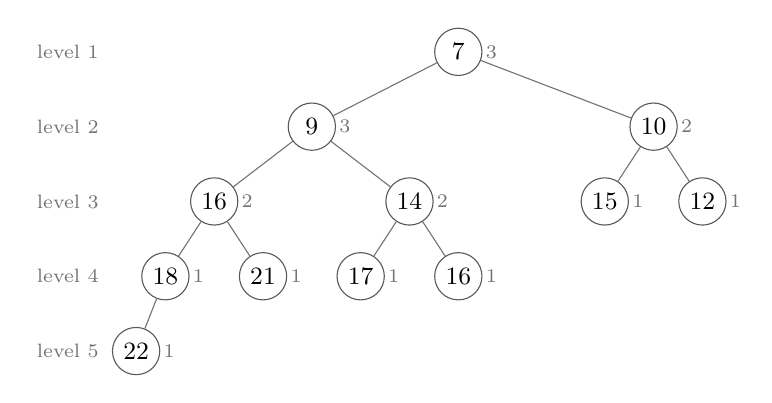
\begin{tikzpicture}[x=0.62cm,y=0.95cm,
  ln/.style={circle, draw=black!65, minimum size=0.6cm, inner sep=0pt, font=\small},
  le/.style={draw=black!55},
  ls/.style={font=\scriptsize, text=black!55, anchor=west, inner sep=1pt}]
\node[ln] (a7) at (6,0) {7};
\node[ln] (a9) at (3,-1) {9};
\node[ln] (a10) at (10,-1) {10};
\node[ln] (a16) at (1,-2) {16};
\node[ln] (a14) at (5,-2) {14};
\node[ln] (a15) at (9,-2) {15};
\node[ln] (a12) at (11,-2) {12};
\node[ln] (a18) at (0,-3) {18};
\node[ln] (a21) at (2,-3) {21};
\node[ln] (a17) at (4,-3) {17};
\node[ln] (a16b) at (6,-3) {16};
\node[ln] (a22) at (-0.6,-4) {22};
\draw[le] (a7)--(a9) (a7)--(a10) (a9)--(a16) (a9)--(a14) (a10)--(a15) (a10)--(a12)
  (a16)--(a18) (a16)--(a21) (a14)--(a17) (a14)--(a16b) (a18)--(a22);
\foreach \n/\s in {a7/3, a9/3, a10/2, a16/2, a14/2, a15/1, a12/1, a18/1, a21/1, a17/1, a16b/1, a22/1}
  \node[ls] at (\n.east) {\s};
\foreach \y/\l in {0/1, -1/2, -2/3, -3/4, -4/5} \node[font=\scriptsize, text=black!55] at (-2,\y) {level \l};
\end{tikzpicture}
\end{center}

逐項檢查：
\begin{itemize}
\item (A) 錯。 根 $7$ 的右子樹是 $10, 15, 12$，只有 $3$ 個節點；其他 $8$ 個節點都在左子樹。
\item (B) 對。 $15$ 的路徑是 $7 \to 10 \to 15$，在第 $3$ 層。
\item (C) 錯。 根到最近的外部節點，例如 $7 \to 10 \to 12 \to$ 空位，要經過 $s(7) = 3$ 個節點、$3$ 條邊
（資結書定理~8.2：一路往右走剛好經過 $s$ 個節點）。 $2$ 條邊只能走到葉節點 $12$，還沒到外部節點。
\item (D) 錯。 兩個 $16$（$9$ 的左子節點、$14$ 的右子節點）都在根的左子樹裡。
\end{itemize}
\end{pastsoln}
